% vim: fileencoding=utf-8:tw=0:noexpandtab:ts=4:sw=4
% -*- coding: utf-8 -*-

\documentclass{svmult}

% packages from template
\usepackage{mathptmx}       % selects Times Roman as basic font
\usepackage{helvet}         % selects Helvetica as sans-serif font
\usepackage{courier}        % selects Courier as typewriter font
\usepackage{makeidx}         % allows index generation
\usepackage{graphicx}        % standard LaTeX graphics tool
                             % when including figure files
\usepackage{multicol}        % used for the two-column index
\usepackage[bottom]{footmisc}% places footnotes at page bottom

% other packages
\usepackage[mathletters]{ucs}
\usepackage[utf8x]{inputenc}
\usepackage{graphicx}
\usepackage{microtype}
\usepackage{amsmath}
\usepackage{url}
\usepackage{tabularx}
\usepackage{booktabs}

% options
\graphicspath{{figures/}{generated-figures/}}

% commands
\newcommand{\fig}[1]{Figure~\ref{fig:#1}}
\newcommand{\Fig}[1]{Figure~\ref{fig:#1}}
\newcommand{\tbl}[1]{{Table}~\ref{fig:#1}}
\newcommand{\Tbl}[1]{{Table}~\ref{fig:#1}}
\newcommand{\sect}[1]{Section~\ref{sec:#1}}
\newcommand{\Sect}[1]{Section~\ref{sec:#1}}
\newcommand{\hypo}[1]{Hypothesis~\ref{hyp:#1}}
\newcommand{\Hypo}[1]{Hypothesis~\ref{hyp:#1}}
\newcommand{\algo}[1]{Algorithm~\ref{algo:#1}}
\newcommand{\Algo}[1]{Algorithm~\ref{algo:#1}}
\newcommand{\eq}[1]{Equation~\ref{eq:#1}}
\newcommand{\Eq}[1]{Equation~\ref{eq:#1}}
\newcommand{\ent}[1]{\mathrm{H}_\mathrm{#1}} % entropy (\H already exists :/)


\title*{Localization of inexpensive robots with low-bandwidth sensors}

\author{Shiling Wang and Francis Colas and Ming Liu and Francesco Mondada and Stéphane Magnenat}
\institute{Shiling Wang \at ETH Zürich,	\email{shilingwang0621@gmail.com}
\and Francis Colas \at INRIA Nancy Grand Est, \email{francis.colas@inria.fr}
\and Ming Liu \at City University of Hong Kong, \email{mingliu@cityu.edu.hk}
\and Francesco Mondada \at Mobots, LSRO, EPFL, \email{francesco.mondada@epfl.ch}
\and Stéphane Magnenat \at Mobots, LSRO, EPFL, \email{stephane@magnenat.net}
}

\makeindex             % used for the subject index
                       % please use the style svind.ist with
                       % your makeindex program

\begin{document}

\maketitle

\abstract*{
Recent progress in electronics has allowed the construction of affordable mobile robots.
This opens many new opportunities, in particular in the educational context.
However, for cost reasons these robots have little long-range sensing abilities and bad dead-reckoning capabilities.
This limitation has prevented them from performing global localization without external aids.
This severely limits their use, for example to teach spatial reasoning or develop artistic activities.
In this paper, we propose a solution to this problem, using only approximate dead-reckoning and infrared sensors measuring the grayscale intensity of a known visual pattern on the ground.
Our approach builds on a recursive Bayesian filter, of which we demonstrate two implementations: a dense Markov Localization and a particle-based Monte Carlo Localization.
We show that both implementations allow accurate localization on a large variety of patterns, from pseudo-random black and white matrices to grayscale drawings by children.
We provide a theoretical estimate and an empirical validation of the necessary traveled distance for convergence.
We demonstrate the real-time localization of a Thymio~II robot.
These results show that our system solves the problem of absolute localization of inexpensive robots.
This enables a new range of educational activities, which strongly increases the value of robots for education.
}

\section{Introduction}

Driven by consumer products, the technologies of electronics, motor and battery have made tremendous progress in the last decades.
They are now widely available at prices making affordable mobile robots a reality.
This opens many new opportunities, in particular in the contexts of collective robotics and education.

Collective and swarm robotics focus on the scalability of systems when the number of robots increases.
In that context, global localization is a challenge, whose solution depends on the environment the robots evolve in.
A common approach is to measure the distance and orientation between robots~\cite{prorok2012low}, but this approach relies on beacons to provide absolute measurements.
Yet, several state of the art algorithms require global positionning~\cite{breitenmoser2016combining}.
In experimental work, it is often provided by an external system, bringing a non-scalable single point of failure into the system, and breaking the distributed aspect.
Therefore, there is the need for a distributed and affordable global localisation system for collective robotics experiments.

In the context of education, robots have been shown to be effective in supporting the teaching of knowledge in fields such as mathematics, physics, computer science and engineering; and of skills such as problem solving and introduction to the scientific method~\cite{benitti2012explorin}.
These fields deal with distances and angles and would profit from localization capabilities.
Similarly, while robots have the potential to reach minorities currently under-represented in technical fields, they typically do so through art and storytelling~\cite{szecsei2015girls}.
Such educational activities, for example staging a theater play with robots, would typically benefit from having absolute positioning.
Yet, all affordable general-public educational robots (in the 100\,\$ range) lack the necessary long-range sensing or precise dead-reckoning capabilities to achieve localization.
Indeed, on platforms that must already provide a variety of programming and sensing modalities to meet general educational needs, proper wheel encoders are still too expensive.

% \begin{figure}
% 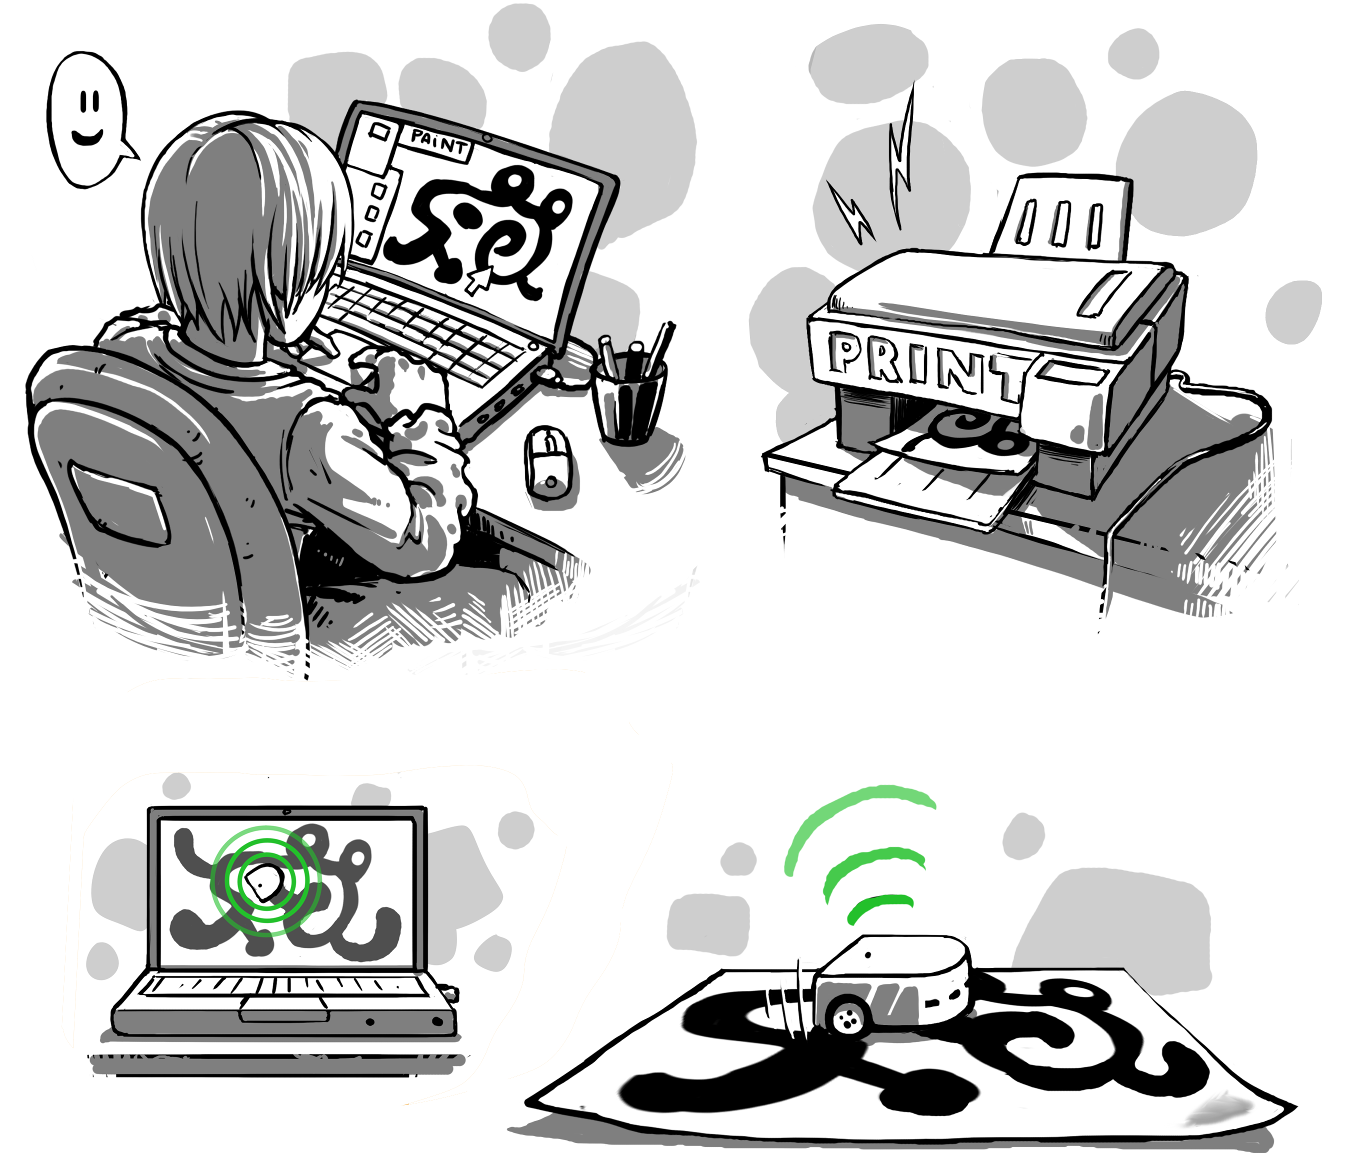
\includegraphics[width=\columnwidth]{process_creation_col_small}
% \caption{The process of creating a ground drawing serving as the map.}
% \label{fig:process}
% \end{figure}

This paper answers the need of affordable absolute positioning by providing a system using only approximate dead-reckoning and inexpensive infrared sensors measuring the grayscale intensity of the ground, without knowing the initial pose of the robot.
The ground can be an existing image or a drawing created by the child herself (\fig{thymio}, left).
Our solution is based on the classical Markov~\cite{fox1999markov} and Monte Carlo~\cite{dellaert1999monte} Localization frameworks that can be seen as respectively a dense and a sampling-based implementation of a recursive Bayesian filter.
While these approaches are commonly used in robots with extensive sensing capabilities such as laser scanners, their implementation on extremely low bandwidth sensors is novel, and rises specific questions, such as which distance the robot must travel for the localization to converge.

In this paper, we deploy these algorithms on the Thymio~II differential-wheeled mobile robot.
The robot reads the intensity of the ground using two infrared sensors (\fig{thymio}, middle, circled red) and estimates the speed of its wheels by measuring the back electromotive force, which is less precise than encoder-based methods.
A Vicon tracking system (\url{http://www.vicon.com/}) provides the ground-truth pose (\fig{thymio}, right).
Our first contribution is a predictive model of the necessary distance to travel to localize the robot.
Our second contribution is a detailed analysis of the performances of the two implementations in comparison with ground-truth data.
Our last contribution is a validation of real-time localization.

\begin{figure}
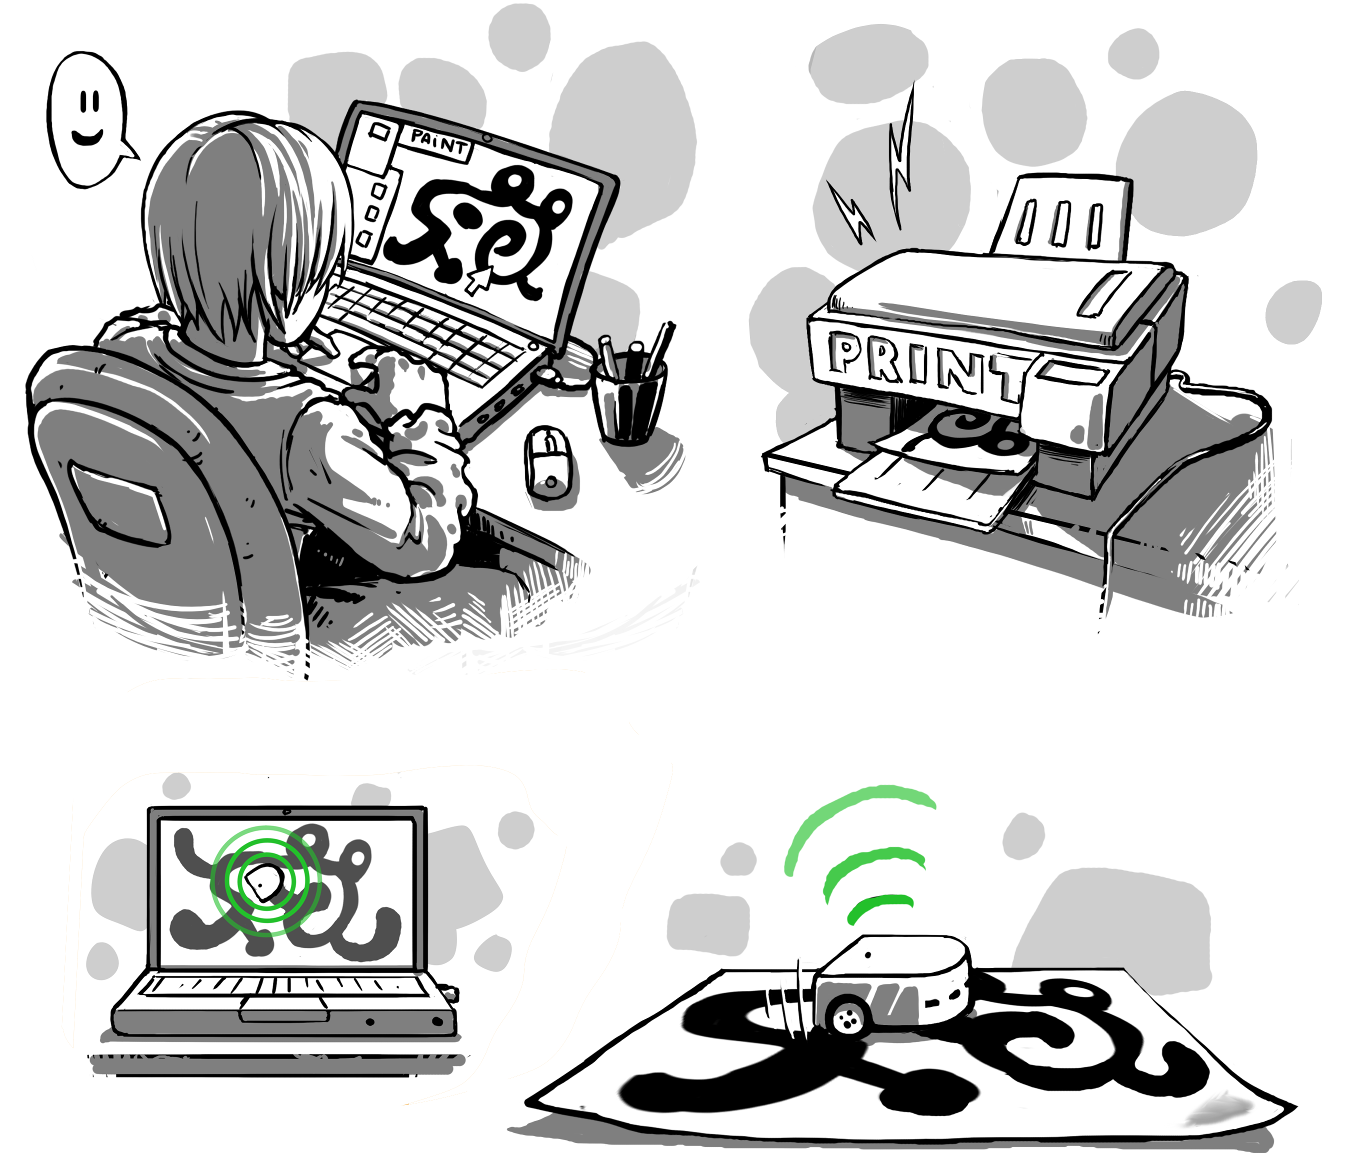
\includegraphics[height=.27\columnwidth]{process_creation_col_small}\hfill
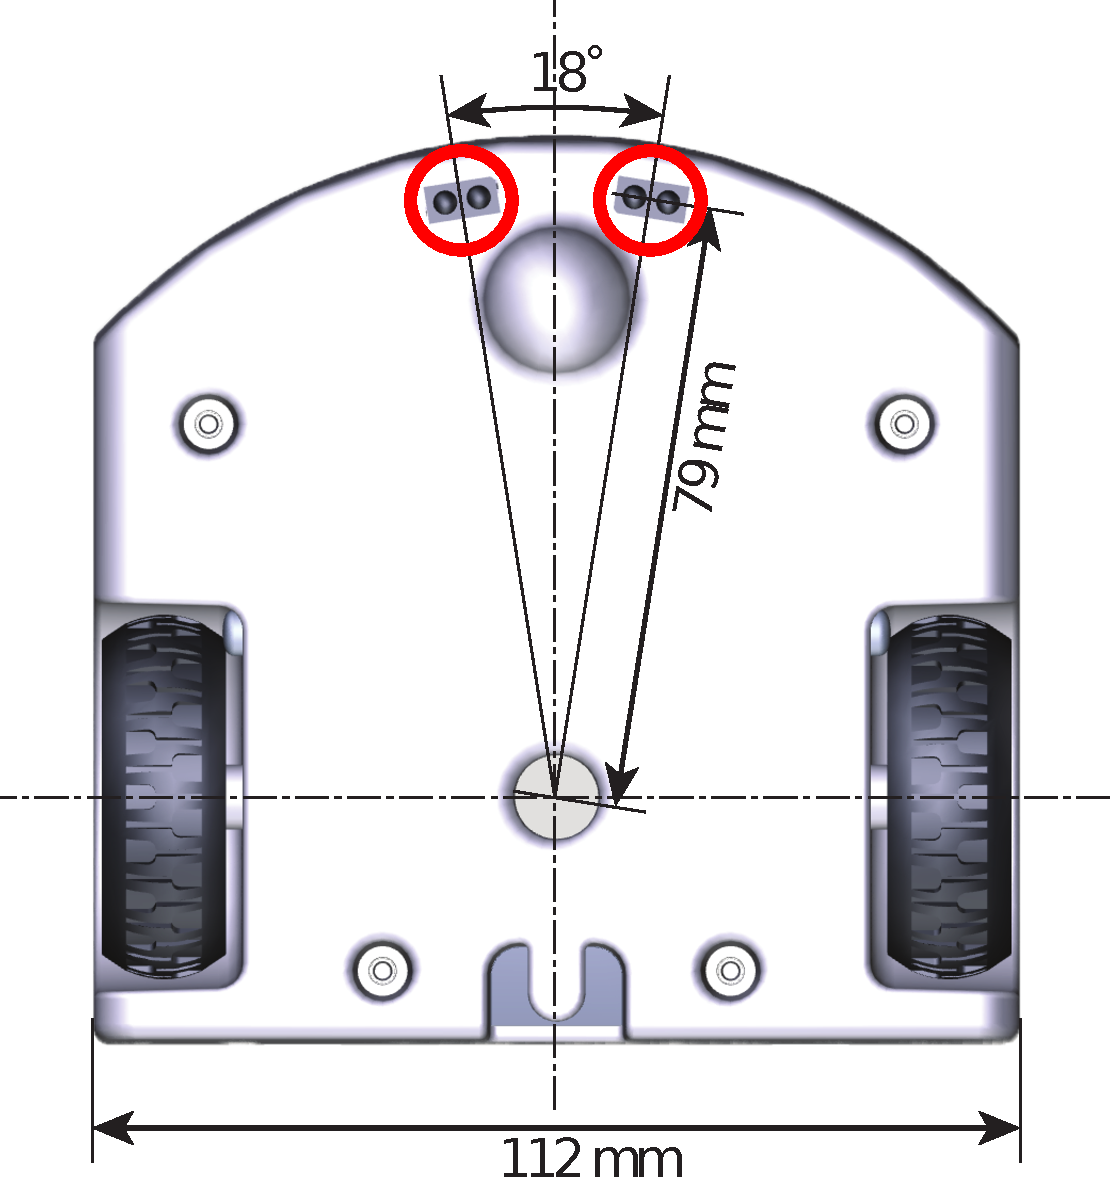
\includegraphics[height=.27\columnwidth]{thymio2-dimensions}\hfill
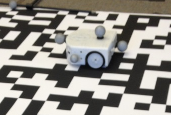
\includegraphics[height=.27\columnwidth]{thymio2-dataset}
\vspace{-.07cm}
\caption{The process of creating a ground drawing serving as the map (left), the Thymio~II robot with the placement of its ground sensors (middle), and markers for tracking its ground-truth pose by a Vicon system (right).}
\label{fig:thymio}
\end{figure}

\section{Related work}

The main challenge of solving the localization problem on affordable mobile robots is the limited information content typical inexpensive sensors can provide.

Zug et al.~\cite{zug2011design} have developed an algorithm using an array of triangulation-based infrared distance sensors.
A Kalman filter algorithm is applied to localize the robot within a 2 by 1\,m box.
No experimental result is provided, but a simulation shows the estimated error to be within 2\,cm.
Pinto et al.~\cite{pinto2012localization} have developed a localization system using wheel encoders and infrared distance sensors, in the context of education.
They mount the sensor on a platform built around a LEGO Mindstorms NXT and use an Extended Kalman Filter for localization.
However, they do not provide experimental result either.

Focusing on a low cost, Gutmann et al.~\cite{gutmann2013challenges} have developed a system using only 3 or 4 light detectors, able to localize a mobile robot in a room with an accuracy of 10\,cm.
Their system is based on detecting a known pattern projected on the ceiling and fusing this information with odometry.
However, this method demands the installation of a projector and requires empty space over it.

Park and Hashimoto~\cite{park2009approach} proposed to localize a mobile robot over a ground equipped with randomly distributed passive \textsc{rfid} tags.
The average localization error of this method is lower than 10\,cm.
However, this approach requires the ground to be equipped, and is only applicable when the starting position of the robot is known.

In the context of education, Singh and Bedi~\cite{singh2013map} have used the ultrasound sensor of the LEGO Mindstorms NXT to localize a robot in a room.
They use a Monte Carlo Localization approach based on a particle filter.
However, they do not provide quantitative results.

Dias and Ventura~\cite{dias2013absolute} use two horizontal lines from a \textsc{vga} camera to read barcodes on the walls of an arena and localize an e-puck robot.
Their system employs an Extended Kalman Filter algorithm and reaches a precision of 1\,cm and 5°.
As with the work of Singh and Bedi, it requires an enclosed arena with a specific wall arrangement and no obstacles between the robot and the walls.

The work of Kurazume and Nagata~\cite{kurazume1994cooperative} first raised the idea of performing inexpensive localization through the cooperative positioning of multiple robots.
Prorok et al.~\cite{prorok2012low} is a modern work representative of this approach.
These authors have used an infrared-based range and bearing hardware along with a distributed Monte Carlo Localization approach, allowing a group of robots to localize down to a precision of 20\,cm.
However, this line of research focuses on scalability rather than absolute positioning, as the later would require fixed robots acting as beacons.
In addition, both radio and infrared-based range and bearing systems require complex electronics.
Finally, when the cost of all robots is added, the system is far from cheap.

To the best of our knowledge, there exist no localization system that uses only a low number of\,--\,or a single\,--\,inexpensive onboard infrared sensor(s), and able to provide absolute positioning.
The system proposed in this paper meets these requirements.

\section{Model}

% old hat, before compression:
% In this section, we start by presenting the generic Bayesian filter used to estimate the pose of the robot in the environment.
% Then we discuss the specificities of the Markov Localization and Monte Carlo Localization approaches for its inference.
% Finally, we propose a theoretical analysis from an information theoretic point of view to give a lower bound on the time or distance to start achieving localization.

%\subsection{Pose estimation filter}
%\subsection{Variables}

The generic Bayesian filter used to estimate the pose of a robot in its environment uses the following variables:
\begin{itemize}
\item $X_{1:t}$ 2-D pose at times $1..t$, consisting of $x,y$ coordinates and an angle $\theta$.
\item $Z_{1:t}$ observations at times $1..t$, consisting of the output of the sensors measuring the grayscale intensity of the ground.
\item $U_{1:t}$ odometry at times $1..t$, consisting of the left and right wheel speeds.
\end{itemize}

%\subsection{Joint probability}
It is classically formulated as a recursive Bayesian filter with the following joint probability distribution:
\begin{equation}
\begin{split}
p(X_{1:t}, Z_{1:t}, U_{1:t}) = p(Z_t|X_t) p(X_t|X_{t-1}, U_{t}) p(U_t) p(X_{1:t-1}, Z_{1:t-1}, U_{1:t-1}).
\end{split}
\end{equation}

%\subsection{Question}
This joint probability distribution allows to formulate the problem as the estimation of the pose $X_t$ at time $t$ given the observations $Z_{1:t}$ and the commands $U_{1:t}$:
\begin{equation}
p(X_t|Z_{1:t},U_{1:t}) \propto p(Z_t | X_t) \sum_{X_{t-1}} p(X_t|X_{t-1}, U_t) p(X_{t-1} | Z_{1:t-1}, U_{1:t-1}).
% = \frac{p(X_t,Z_t | Z_{1:t-1}, U_{1:t})}{p(Z_t|Z_{1:t-1}, U_{1:t})} \\
% &\propto p(Z_t | X_t) p(X_t | Z_{1:t-1}, U_{1:t}) \\
% &\propto p(Z_t | X_t) \sum_{X_{t-1}} p(X_t, X_{t-1} | Z_{1:t-1}, U_{1:t} ) \\
\end{equation}
%This is a recursive filter to estimate $X_t$ using the previous estimation $X_{t-1}$, the odometry $U_t$ and the observation $Z_t$.

%\subsection{Distributions}
This inference involves two distributions to specify the \emph{observation model} $p(Z_t | X_t)$ and the \emph{motion model} $p(X_t|X_{t-1}, U_t)$, which are specific to our Thymio~II robot.
In addition, we define a \emph{self-confidence metrics} and outline the implementation.

%\subsubsection{Observation model}

\textbf{Observation model}. Thymio~II has two infrared ground sensors measuring the grayscale value of the ground (\fig{thymio}, center).
%Despite the observations being coupled through the known visual ground pattern serving as map, our model assumes them to be independent, so $p(Z_t | X_t) = \prod_{i=0,1} p(Z_t^{i} | X_t)$.
%Moreover, we assume the ground color to be in the range $[0,1]$ with $0$ being black and $1$ being white.
Our observation model $p(Z_t | X_t) = \prod_{i=0,1} p(Z_t^{i} | X_t)$ assumes these two sensors to be independent, and the ground color to be in the range of $[0,1]$ ($0$ being black and $1$ being white).
%Hence, if sensor $i$ for robot pose $X_t$ should see a ground intensity $v$ according to the map, $p(Z_t^{i} | X_t) \sim \mathcal{N}(v,\sigma_\mathrm{obs})$.
Hence $p(Z_t^{i} | X_t) \sim \mathcal{N}(v,\sigma_\mathrm{obs})$, for robot pose $X_t$, sensor $i$, and a corresponding ground intensity $v$ according to the map.
The parameter $\sigma_\mathrm{obs}$ is selected based on the knowledge of the sensor.
For black and white patterns, we assume the probability of seeing the correct color when the value measured by the sensor corresponds to the one in the map to be $p_\mathrm{correct} = 0.95$, leading to $\sigma_\mathrm{obs} = 0.5$.
For grayscale images, based on measurement on a real Thymio~II, we set $\sigma_\mathrm{obs}$ to $0.15$.

%\subsubsection{Motion model}

\textbf{Motion model}. Based on the model of Eliazar et al.~\cite{eliazar2004motionmodel}, we assume that the motion has a Gaussian error model, hence $p(X_t~|~X_{t-1}, U_{t})\sim\mathcal{N}(\mu_t,\Sigma_t)$.
The mean $\mu_t$ is built by accumulating the estimated displacements by dead-reckoning between times $t-1$ and $t$.
Therefore, if $\Delta x_t$, $\Delta y_t$, $\Delta \theta_t$ are the displacement between $t-1$ and $t$, expressed in the robot local frame at $t-1$, $\mu_t$ is:
\begin{equation}
\mu_t =
\left[ \begin{array}{c} x_t \\ y_t \\ \theta_t \end{array} \right]
\text{with}
\begin{array}{c}
\left[ \begin{array}{c} x_t \\ y_t \end{array} \right] =
\left[ \begin{array}{c} x_{t-1} \\ y_{t-1} \end{array} \right] +
R(\theta_{t-1})
\left[ \begin{array}{c} \Delta x_{t} \\ \Delta y_{t} \end{array} \right]
\\
\theta_t = \theta_{t-1} + \Delta \theta_t
\end{array}
\end{equation}
where $R(\theta)$ is the 2-D rotation matrix of angle $\theta$.
The $3\times3$ diagonal covariance matrix $\Sigma_t$ is a function of the distance traveled, the amount of rotation, and two parameters $\alpha_\mathrm{xy}$, $\alpha_\theta$:
\begin{equation}
\Sigma_t=\begin{bmatrix} \sigma_{\mathrm{xy},t}^2 & 0 & 0 \\ 0 & \sigma_{\mathrm{xy},t}^2 & 0 \\ 0 & 0 & (\alpha_\theta | \Delta \theta_t |)^2 \end{bmatrix}
\end{equation}
with $ \sigma_{\mathrm{xy},t} = \alpha_\mathrm{xy} \sqrt{\Delta x_{t}^2 + \Delta y_{t}^2}$.

In addition, to cope for the possibility of the robot being kidnapped and therefore its pose becoming unknown, a uniform distribution with a weight $p_\mathrm{uniform}$ is added to $X_t$.
The parameters $\alpha_\mathrm{xy}$, $\alpha_\theta$ and $p_\mathrm{uniform}$ are estimated using maximum likelihood (see \sect{mle}).

%\subsubsection{Self confidence}

\textbf{Self confidence}. We define a self-confidence term that corresponds to the ratio of the probability mass of $p(X_t)$ that is within a distance $d_\mathrm{xy}$ and an angle difference $d_\theta$ to the estimated pose.
We use $d_\mathrm{xy} = 3$\,cm and $d_\theta = 10$°.

%\subsection{Implementations}

\textbf{Implementations}.
We compare two variants of this filter.
In Markov Localization, the distributions are discretized using regular grids~\cite{fox1999markov}.
For our experiments, the $x,y$ cell resolution is 1\,cm and the angular resolution varies from 20° (18 discretization steps for 360°) to 5° (72 discretization steps for 360°).
The estimated pose is the coordinates of the cell of maximum probability.
In Monte Carlo Localization~\cite{dellaert1999monte}, the distributions are represented using samples in a particle filter.
In order to extract a single pose estimate out of the many particles, we find a maximum density area in which we average the particles.
It is similar to a 1-point \textsc{ransac} scheme~\cite{Fischler1981ransac}.
%Both the search for the particle with most neighbors and the search for neighbors are done with 500 trials.
%The thresholds for a particle to be a neighbor are a distance of 1.5\,cm and an angular difference of 5°.
We implemented both algorithms in Python with some Cython (\url{http://www.cython.org}) procedures used for time-critical inner loops.
Thymio~II is programmed through the \textsc{aseba} framework~\cite{aseba2011tmech}, which connects to Python using D-Bus.

\section{Theoretical analysis of convergence}
\label{sec:theoreticalconv}

It is possible to estimate the time required for the robot to localize itself in a given known space.
For the Markov Localization approach, there is a given number of discrete cells.
The amount of information needed to unambiguously specify one among them all is $\ent{loc} = \log_2(N_\mathrm{cells})$, with $N_\mathrm{cells}$ the number of cells.

We can also estimate the information gain at each time step.
Let us consider the case of a binary map and a binary sensor.
This sensor ideally yields 1\,bit of information per measurement.
However in practice, there is a loss in information due to the sensor noise, characterized by the $p_\mathrm{correct}$ probability of the sensor to be correct:
\begin{equation}
	\ent{noise} = \ent{b}(1 - p_\mathrm{correct}),
\end{equation}
where $\ent{b}$ is the binary entropy function: $\ent{b}(p) = -p\log_2(p) - (1-p)\log_2(1-p)$.

In addition, we need to take into account that our sensor measurements are not completely independent.
For example, when not moving, we always observe the same place and thus cannot really gain additional information besides being sure of the intensity of the current pixel.
In a discretized world, we thus need to estimate the probability of having changed cell in order to observe something new, which depends on the distance traveled and the size of the cells.
This problem is equivalent to the Buffon-Laplace needle problem of finding the probability for a needle thrown randomly on a grid to actually intersect the grid~\cite{laplace1820prob}.
In our case, the probability of changing cell is given by:
\begin{equation}
	p_\mathrm{diff} = \frac{4d h - d^2}{\pi h^2},
\end{equation}
with $d$ the distance traveled and $h$ the size of the cells.

We can then compute the conditional entropy for two successive ideal binary measurements $O_{t-1}$ and $O_t$ separated by $d$ based on the conditional probability.
There are two cases: either the robot has not moved enough to change cell (with probability $1 - p_\mathrm{diff}$) and the new observation is the same as the old, or the robot has changed cell (with probability $p_\mathrm{diff}$) and the new observation has the same probability to be the same or the opposite of the old.
This can be summarized by the following conditional probability distribution:
\begin{equation}
\begin{split}
	&p(O_t=\{\mathrm{black}/\mathrm{white}\} \mid O_{t-1}=\{\mathrm{black}/\mathrm{white}\})\\
	&= \begin{pmatrix}
		(1 - p_\mathrm{diff}) + p_\mathrm{diff}/2 & p_\mathrm{diff}/2\\
		p_\mathrm{diff}/2 & (1 - p_\mathrm{diff}) + p_\mathrm{diff}/2
	\end{pmatrix}
\end{split}
\end{equation}
After rearranging the terms of the conditional entropy, the loss of information due to redundancy in the traveled distance is:
\begin{equation}
	\ent{loss,d} = 1 - \ent{b}(p_\mathrm{diff}/2).
\end{equation}

There is also redundancy between several sensors placed on the same robot.
The probability that they see the same cell based on the distance between them is exactly the same as the probability of a sensor to see the same cell after a displacement of the same distance.
The information loss due to the redundancy from the sensor placement is noted $\ent{sensors}$ and follows the same formula as $\ent{loss,d}$ for the distance between the two sensors.

Finally, we can approximate the information that our robot gathers at each time step by assuming that the trajectory of the robot does not loop (no redundancy between distant time steps) and that the trajectories of the sensors are independent. 
The information gathered in a time step is then:
\begin{equation}
\begin{split}
	\ent{}(O^1_t, O^2_t \mid O^1_{1:t-1}, O^2_{1:t-1}) &= \ent{}(O^1_t, O^2_t \mid O^1_{t-1}, O^2_{t-1}) \\
	&= \ent{}(O^1_t \mid O^1_{t-1}) + \ent{}(O^2_t \mid O^2_{t-1}) - \ent{}(O^2_t \mid O^1_t) \\
	&= 2\cdot(1-\ent{noise}-\ent{loss,d}) - \ent{sensors}%. The full stop here is ugly.
\end{split}
\end{equation}
This formula also ignores the uncertainty in the robot motion.
With these assumptions, it is an upper bound on the average information gain.

In our example, we have assumed $p_\mathrm{correct}=0.95$, that is $\ent{noise}=0.29$.
Our robot moves at 3\,cm/s with a time step of 0.3\,s and 3\,cm cells in which the color is known to be similar; this yields $p_\mathrm{diff}=0.35$ and $\ent{loss,d}=0.33$.
Finally the sensors are 2.2\,cm apart which yields $p_\mathrm{diff}=0.76$ and $\ent{sensors}=0.041$.
As such the robot gathers on average at most 0.72\,bit per time step, or 0.8\,bit/cm.

With a 150\,cm$\times$150\,cm environment discretized with cells of 1\,cm and 5° angle, the amount of information needed for the localization is $\ent{loc}=20.6$.
This means that, on average, the robot should not be localized before traveling around 26\,cm.

Faster localization can be achieved by moving at a greater speed to reduce redundancy in the successive measurements.
If designing a new robot, better sensors would reduce cross-over noise.
Setting the sensors apart would also reduce the redundancy between their information but, for our specific grid size, they are sufficiently separated in Thymio~II.

\section{Empirical analysis of performance}

% \begin{figure}
% 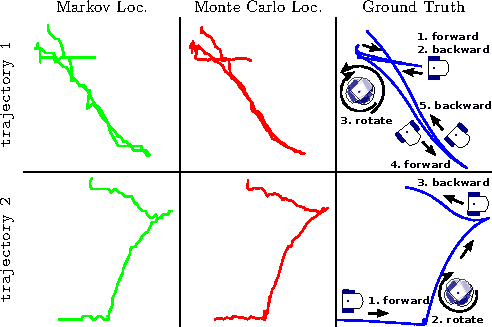
\includegraphics{trajectories}
% \caption{The estimations (after convergence) along with the ground truth for the two first trajectories.
% For Markov Localization, the angle discretization is 72; for Monte Carlo Localization, there are 400k particles.
% }
% \label{fig:trajectories}
% \end{figure}

To evaluate the performance of our localization algorithms, we remotely controlled the robot and recorded datasets covering all possible robot motions:
\begin{itemize}
\item \texttt{trajectory 1} and \texttt{2}: The robot alternates forward and backward movements with rotations on spot, at a speed of 3--5\,cm/s. % (see \fig{trajectories}).
%\item \texttt{linear trajectory}: The robot simply goes straight ahead along the x-axis of the map, at a speed of 3--5\,cm/s.
\item \texttt{trajectory with kidnapping}: The robot alternates phases of forward movement, at a speed of 15\,cm/s, and turning on spot.
To test the algorithm's ability of recovering from catastrophic localization failures, we perform ``robot kidnapping'' by lifting the robot and moving it to another part of the map every minute.
\end{itemize}
The robot moves on a 150$\times$150\,cm ground pattern containing 50\,$\times$\,50 cells of 3$\times$3\,cm, each randomly black or white (\fig{thymio}, right).
The robot is connected to \textsc{ros}\footnote{ROS (Robot Operating System): \url{http://www.ros.org/}} to synchronize its sensor values and odometry information with ground-truth data from Vicon.
%to provide the ground-truth robot pose, consisting of $x$, $y$ coordinates and the heading $\theta$.
The data are gathered with a frequency of 100\,Hz (ground-truth) and 10\,Hz (robot) and subsequently down-sampled to a period of 0.3\,s.
We chose this period so that with basic trajectories, at maximum speed the robot travels approximately half the length of one cell between every sample.

%\subsection{Parameter estimation}
\label{sec:mle}

\textbf{Parameter estimation}.
The noise parameters of the motion model were estimated using maximum likelihood, considering the error between the ground truth and the odometry data in the local frame between two time steps.
Using \texttt{trajectory~1} and \texttt{trajectory~2}, the values for  $\alpha_\mathrm{xy}$ and $\alpha_\theta$ were found be in the order of 0.1.
Similarly, using \texttt{trajectory with kidnapping}, the value for $p_\mathrm{uniform}$ was also found to be in the order of 0.1.

%\subsection{Basic localization}

\begin{figure*}

\begin{center}
Markov Localization, for different \emph{number of discretization angles}
\end{center}
\begin{minipage}{.5\columnwidth}
\begin{center}
\texttt{trajectory~1}
\end{center}
\end{minipage}
\hfill
\begin{minipage}{.5\columnwidth}
\begin{center}
\texttt{trajectory~2}
\end{center}
\end{minipage}

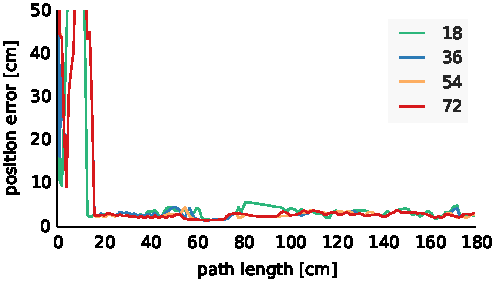
\includegraphics[width=.24\columnwidth]{ml-whole_random_1-xy}\hfill
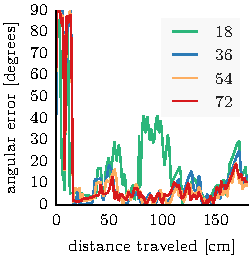
\includegraphics[width=.24\columnwidth]{ml-whole_random_1-theta}\hfill
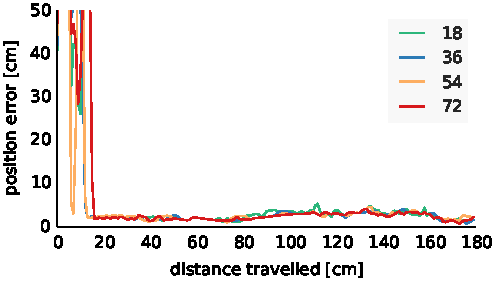
\includegraphics[width=.24\columnwidth]{ml-whole_random_2-xy}\hfill
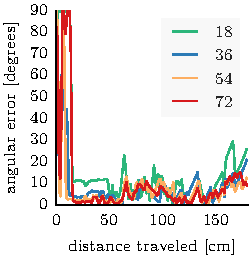
\includegraphics[width=.24\columnwidth]{ml-whole_random_2-theta}

\vspace{.3em}

\begin{center}
Monte Carlo Localization, for different \emph{number of particles}
\end{center}
\begin{minipage}{.5\columnwidth}
\begin{center}
\texttt{trajectory~1}
\end{center}
\end{minipage}
\hfill
\begin{minipage}{.5\columnwidth}
\begin{center}
\texttt{trajectory~2}
\end{center}
\end{minipage}


\vspace{.3em}

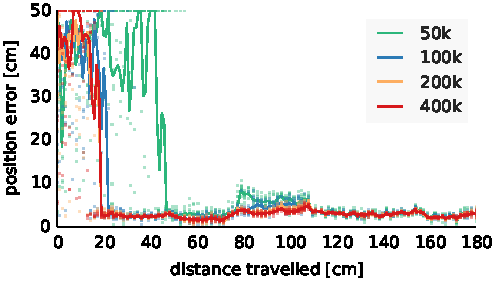
\includegraphics[width=.24\columnwidth]{mcl-whole_random_1-xy}\hfill
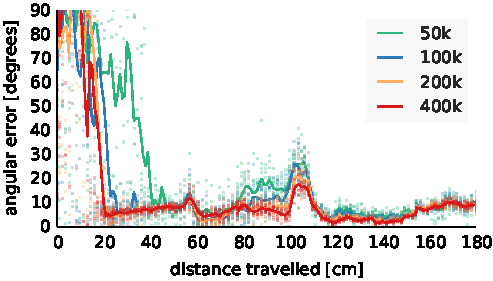
\includegraphics[width=.24\columnwidth]{mcl-whole_random_1-theta}\hfill
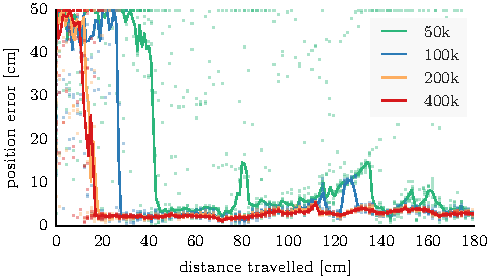
\includegraphics[width=.24\columnwidth]{mcl-whole_random_2-xy}\hfill
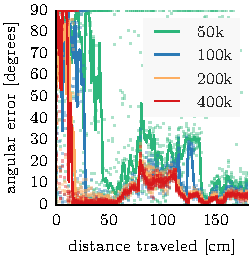
\includegraphics[width=.24\columnwidth]{mcl-whole_random_2-theta}

\caption{The error between the estimation by the localization algorithm and the ground truth on \texttt{trajectory~1} and \texttt{trajectory~2}.
For Monte Carlo Localization, the solid lines show the average over 10 trials, while the light dots show the individual trials.}
\label{fig:whole-runs-random12}
\end{figure*}

\textbf{Basic localization}.
\Fig{whole-runs-random12} shows the error in position and orientation for the first two trajectories.
In these plots, \emph{distance traveled} represents the cumulative distance traveled by the center point between the two ground sensors of the robot.
The error is clamped at 50\,cm for position and 90° for orientation.

For the Markov Localization approach, all discretization resolutions allow the robot to localize down to a precision of 3\,cm and 5°.
However, in \texttt{trajectory~1}, the resolution of 18 discretization steps is not enough to keep tracking the orientation at a distance traveled of 50\,cm and 80\,cm.
These both correspond to the robot rotating on spot.
Better resolutions do not exhibit this problem and have similar precisions.
Therefore, we see that an angular discretization of 36 (10° resolution) is sufficient to provide accurate tracking, and that a finer resolution only provides minor improvements in angular precision, and no improvement in position precision.
In \texttt{trajectory~2}, we see that a resolution of 54 allows for a better angular precision than 36, but 72 does not improve over 54.
All resolutions provide equal position precision.

For the Monte Carlo Localization approach, we see that on \texttt{trajectory~1}, the robot localizes already with 50k particles, but in twice the time it takes with 100k particles.
Increasing the number of particles beyond this value only marginally decreases localization time.
While 50k particles are sufficient to localize on this run on average, in some runs, the robot loses orientation when it turns on spot.
On \texttt{trajectory~2}, 50k particles is not enough to localize the robot.
Increasing this number to 100k leads to a good localization, except after the robot has traveled 130\,cm; which corresponds to a long moment during which the robot rotates on spot, leading to less information acquisition, and therefore degraded precision.

Overall, both approaches have similar localization accuracy.
When angular precision is critical, the Monte Carlo Localization approach might achieve better performance, as the Markov Localization approach is limited in precision by its discretization.

%\subsection{Distance to converge}

\begin{figure}

\begin{minipage}{.5\columnwidth}
\begin{center}
Markov Localization\\for different \emph{number of discretization angles}
\end{center}
\end{minipage}
\hfill
\begin{minipage}{.5\columnwidth}
\begin{center}
Monte Carlo Localization\\for different \emph{number of particles}
\end{center}
\end{minipage}

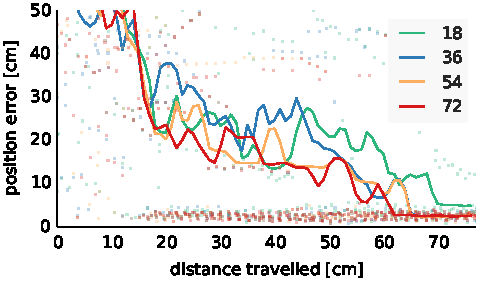
\includegraphics[width=.5\columnwidth]{ml-small_runs_random_12-xy}
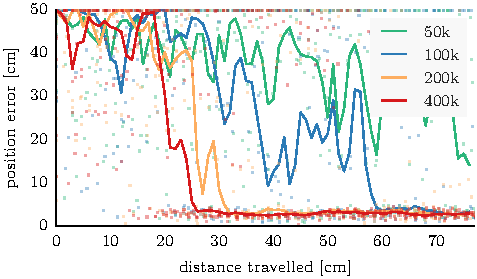
\includegraphics[width=.5\columnwidth]{mcl-small_runs_random_12-xy}

\caption{%
The error between the estimation by the localization algorithm and the ground truth on 10 segments from the first two trajectories.
The solid lines show the median while the light dots show the individual trials.}
\label{fig:small-runs}
\end{figure}

\textbf{Distance to converge}.
\Fig{small-runs} shows the error in position for 5 different locations in each of the first two trajectories.
We see that, with the Markov Localization approach, the correct pose is found after about 20\,cm.
% TODO check that
%This corresponds well to the ideal theoretical distance of 18\,cm computed in \sect{theoreticalconv}.
This is shorter than the 26\,cm distance computed in \sect{theoreticalconv}.
This is probably due to the overestimation of the cross-over noise of the sensor.
A distance of 20\,cm would correspond to noise lower than 3\% instead of 5\% as assumed.
% end TODO
There are also outliers: this happens when the robot is turning on spot, in which case there is not enough information to localize the robot.
The convergence is slower with the Monte Carlo Localization approach, except with 400k particles, in which case it is roughly similar.
Decreasing the number of particles quickly increases the distance needed for convergence, reaching 60\,cm for 100k particles.
Using only 50k particles, some trajectory segments fail to converge, even after 80\,cm length.

% \Fig{small-maps} shows the effect on convergence distance when the map size is reduced.
% The robot runs linearly on one quarter of the map, while the Markov Localization is provided with the whole map, half of it, and a quarter of it.
% We see that reducing the map size does reduce the distance traveled necessary to converge, in accordance to the theory.
% 
% \begin{figure}
% \sidecaption[t]
% 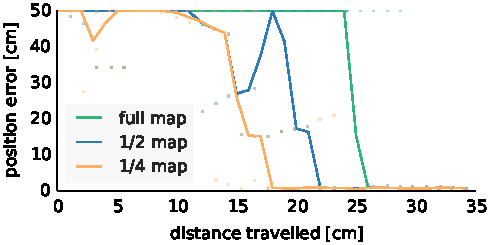
\includegraphics[scale=.9]{ml-small_maps-xy}
% %\vspace{.5em}
% %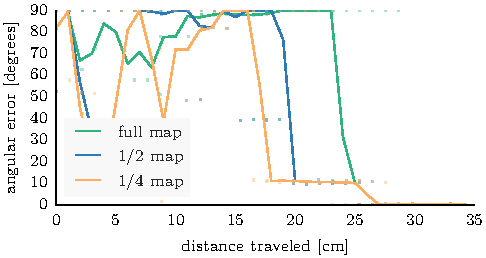
\includegraphics{ml-small_maps-theta}
% \caption{The error between the estimation by the localization algorithm and the ground truth, using Markov Localization, for different map sizes on \texttt{linear trajectory}.
% The solid lines show the median over 3 different trajectory parts, while the light dots show the individual parts.}
% \label{fig:small-maps}
% \end{figure}

%\subsection{Robot kidnapping}

\begin{figure*}

\begin{minipage}{.5\columnwidth}
\begin{center}
Markov Localization\\for different \emph{number of discretization angles}
\end{center}
\end{minipage}
\hfill
\begin{minipage}{.5\columnwidth}
\begin{center}
Monte Carlo Localization\\for different \emph{number of particles}
\end{center}
\end{minipage}

\vspace{.2em}

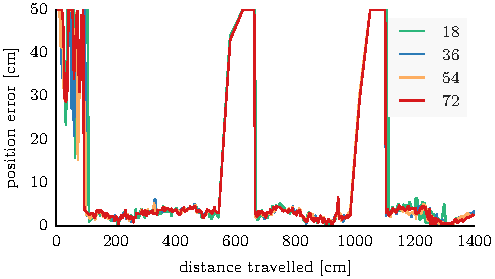
\includegraphics[width=.5\columnwidth]{ml-whole_random_long-xy} \hfill 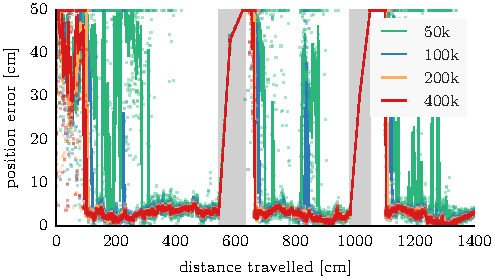
\includegraphics[width=.5\columnwidth]{mcl-whole_random_long-xy}

\vspace{.2em}

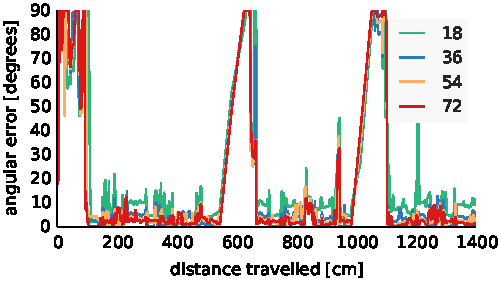
\includegraphics[width=.5\columnwidth]{ml-whole_random_long-theta} \hfill 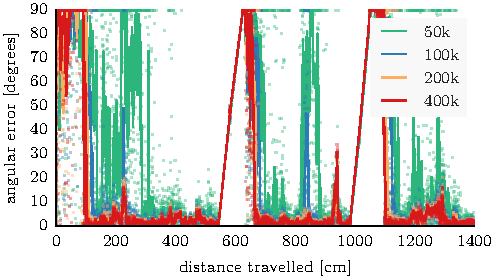
\includegraphics[width=.5\columnwidth]{mcl-whole_random_long-theta}

\vspace{.2em}

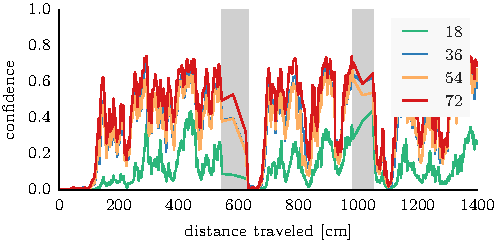
\includegraphics[width=.5\columnwidth]{ml-whole_random_long-conf} \hfill 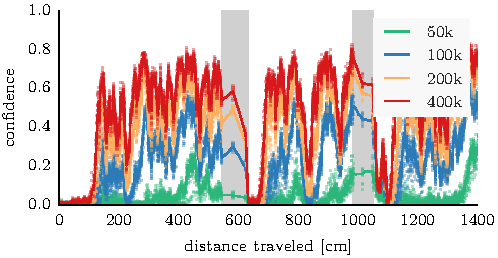
\includegraphics[width=.5\columnwidth]{mcl-whole_random_long-conf}

\caption{The error between the estimation by the localization algorithm and the ground truth, and the self confidence of the algorithm, on the run with kidnapping.
For Monte Carlo Localization, the solid lines show the median over 10 trials, while the light dots show the individual trials.
The gray areas show the time during the robot is being held in the air at the occasion of kidnapping.}
\label{fig:whole-runs-random-long}
\end{figure*}

\textbf{Robot kidnapping}.
\Fig{whole-runs-random-long} shows the error in position, orientation and the self confidence for the run with kidnapping.
In this run, the robot is kidnapped twice, after having traveled 550\,cm and 1000\,cm.
It takes the robot approximately 100\,cm to re-localize, and does so successfully with both Markov and Monte Carlo Localization approaches.
This difference of distance with previous runs is mostly due to the speed of the robot, which is about 5 times faster.
With the Markov Localization approach, all discretization resolutions are approximately equivalent in position performance, but 18 leads to a lower orientation precision, as well as to a lower self confidence, due to the large discretization step.
Other resolutions have a confidence of about 0.5 when the robot is localized, and this value drops below 0.1 after kidnapping, clearly showing that the algorithm is able to assess its status of being lost.

With the Monte Carlo Localization approach, the robot localizes most of the time with 100k particle or more, and always with 200k particles or more.
With 50k particles, the robot eventually localizes, but this might take more than 2 meters of traveled distance.
We see that the self confidence increases with more particles, and also drops after kidnapping, similarly to the Markov Localization approach.
This confirms the effectiveness of the self confidence measure.

%\subsection{Computational cost}

% \begin{figure}
% 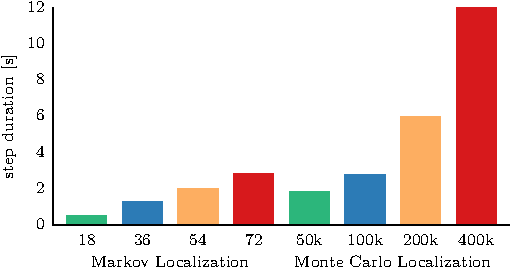
\includegraphics{cpu_load}
% \caption{The execution duration, proportional to the computational cost, for one time step.
% For Markov Localization, the legend indicates the number of discretization steps for angles; for Monte Carlo Localization, the number of particles.
% Data are averaged over all time steps of first two trajectories.}
% \label{fig:cpuload}
% \end{figure}

%\Fig{cpuload} shows the duration of one step for the different algorithms and parameters, averaged over the two first trajectories.

\begin{table}
\noindent \begin{tabularx}{\columnwidth}{l*{4}{>{\centering\arraybackslash}X}|*{4}{>{\centering\arraybackslash}X}}
\toprule
duration [s] & \textbf{0.64} & \textbf{1.43} & \textbf{2.15} & \textbf{2.94} & \textbf{1.97} & \textbf{2.97} & \textbf{6.08} & \textbf{12.22} \\
algorithm & \multicolumn{4}{c}{Markov Localization} & \multicolumn{4}{c}{Monte Carlo Localization} \\
parameter & 18 & 36 & 54 & 72 & 50k & 100k & 200k & 400k \\
& \multicolumn{4}{c}{discretization angles} & \multicolumn{4}{c}{particles} \\
\bottomrule
\end{tabularx}
% ml 18 0.644618824383
% ml 36 1.43336916612
% ml 54 2.14746120327
% ml 72 2.94491757458
% mcl 50k 1.96835128852
% mcl 100k 2.91244221731
% mcl 200k 6.07983028561
% mcl 400k 12.2152938447
\caption{The execution duration of one step for the two algorithms.}
\label{fig:cpuload}
\end{table}

\textbf{Computational cost}.
\Tbl{cpuload} shows the execution duration of one step for the two algorithms with different parameters.
These data were measured on a Lenovo laptop T450s with an Intel Core i7 5600U processor running at 2.6\,GHz, and are averages over the two first trajectories.
We see that with the Markov Localization approach, the duration scales linearly with the number of discretization angles.
With the Monte Carlo Localization approach, the scaling is linear but amortized (50k particles is not twice faster as 100k).
This is due to the selection of pose estimate, which uses a \textsc{ransac} approach and is therefore independent of the number of particles.
For similar localization accuracy, the Monte Carlo Localization approach is slower than the Markov Localization approach, and therefore we suggest to use the former with an angular discretization of 36 in practical applications.
However, the Monte Carlo Localization approach might be preferred if a high angular precision is required, but 100k particles are necessary for proper localization.

% At a computation duration of 1.5\,s per step, the Markov Localization approach with a discretization angle of 36 is far from real time.
% However, this computation duration corresponding to a map size of 150\,cm.
% If the map was smaller, for instance 50\,cm, the algorithm would be 9 times faster.
% Therefore, at 0.15\,s per step, it would be suitable for real-time operations.
% Moreover, the code could be further optimized by using multimedia instructions such as \textsc{sse}, implementing it in the \textsc{gpu}, or parallelizing it.
% Conditional probability tables are well suited for such optimizations.
% The Monte Carlo Localization approach requires at least 100k particle for proper localization, at a computation duration of 2\,s per step.
% While similar optimization is possible, some parts are harder to optimize, in particular the re-sampling step and the \textsc{ransac} step.

\section{Real-time localization}

\begin{figure*}
\makebox[.15\textwidth][c]{Breugel}\hfill
\makebox[.15\textwidth][c]{Van Gogh}\hfill
\makebox[.15\textwidth][c]{Kandinsky}\hfill
\makebox[.15\textwidth][c]{Vermeer}\hfill
\makebox[.15\textwidth][c]{Babar}\hfill
\makebox[.15\textwidth][c]{Child's drawing}

\vspace{.6em}

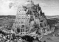
\includegraphics[width=.15\textwidth,interpolate=false]{maps/breugel_babel_A2} \hfill
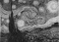
\includegraphics[width=.15\textwidth,interpolate=false]{maps/van-gogh_starry-night_A2} \hfill
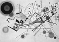
\includegraphics[width=.15\textwidth,interpolate=false]{maps/kandinsky_comp-8_A2} \hfill
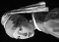
\includegraphics[width=.15\textwidth,interpolate=false]{maps/vermeer_girl-pearl_A2} \hfill
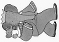
\includegraphics[width=.15\textwidth,interpolate=false]{maps/babar_A2} \hfill
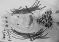
\includegraphics[width=.15\textwidth,interpolate=false]{maps/child-drawing_tooth-fairy_A2}

\vspace{.7em}

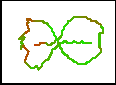
\includegraphics[width=.15\textwidth]{breugel_babel-traj} \hfill
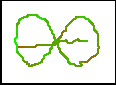
\includegraphics[width=.15\textwidth]{van-gogh_starry-night-traj} \hfill
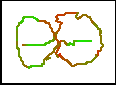
\includegraphics[width=.15\textwidth]{kandinsky_comp-8-traj} \hfill
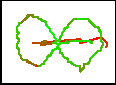
\includegraphics[width=.15\textwidth]{vermeer_girl-pearl-traj} \hfill
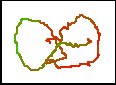
\includegraphics[width=.15\textwidth]{babar-traj} \hfill
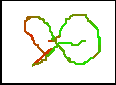
\includegraphics[width=.15\textwidth]{child-drawing_tooth-fairy-traj}

\vspace{.7em}

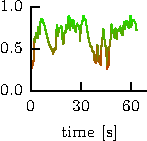
\includegraphics[width=.15\textwidth]{breugel_babel-conf} \hfill
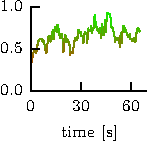
\includegraphics[width=.15\textwidth]{van-gogh_starry-night-conf} \hfill
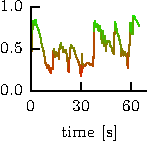
\includegraphics[width=.15\textwidth]{kandinsky_comp-8-conf} \hfill
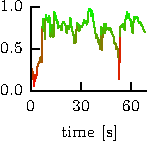
\includegraphics[width=.15\textwidth]{vermeer_girl-pearl-conf} \hfill
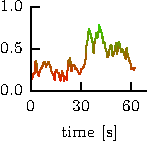
\includegraphics[width=.15\textwidth]{babar-conf} \hfill
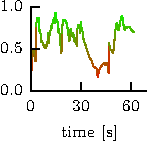
\includegraphics[width=.15\textwidth]{child-drawing_tooth-fairy-conf}

\caption{The image, estimated trajectory and self confidence for different 59\,$\times$\,42\,cm grayscale patterns printed on A2 papers with a resolution of 1\,pixel/cm.
The robot is remotely controlled to draw a 8-shape figure, with similar motor commands for each image.
Markov Localization with 36 discretization angles used.
The color of the lines vary from red (confidence 0) to green (confidence 1).
Trajectories are plotted starting from a confidence level of 0.2.}
\label{fig:a2_drawings}

\end{figure*}

\Fig{a2_drawings} shows the performance of the real-time localization of a Wireless Thymio~II using different grayscale images of 59\,$\times$\,42\,cm, printed on A2 paper sheets with a resolution of 1\,pixel/cm.
We used Markov Localization with an angular discretization of 36 and a spatial resolution of 1\,cm; the localization is performed every 0.4\,s.
The localization algorithm runs on a Lenovo laptop X1 3rd generation with an Intel Core i7-5500U processor running at 2.4\,GHz, at a \textsc{cpu} load of approximately 80\,\%.
The laptop receives the sensor readings from the robot through a wireless connection.
The algorithm localizes the robot globally on all images.
The images with more contrast lead to a more robust and faster localization, while the ones with lower contrast lead to more imprecise trajectories.
The parts of trajectories in red are typically less precise than the ones in green.
This shows that the self confidence measure is effective in assessing the quality of the localization.

\section{Conclusion}

In this paper, we have conducted an empirical evaluation of Markov- and Monte Carlo-based approaches for localizing a mobile robot on a known ground visual pattern.
The robot requires only inexpensive infrared sensors and approximate odometry information.
We have shown that both approaches allow successful localization without knowing the initial pose of the robot, and that their performances and computational requirements are of a similar order of magnitude.
Real-time localization was successful with a large variety of A2 grayscale images, using the Markov Localization approach with 36 discretization steps for angle.
Should larger patterns be desired, the code could be further optimized by using multimedia instructions such as \textsc{sse}, implementing it in the \textsc{gpu}, or parallelizing it.
%Conditional probability tables are well suited for such optimizations.

In addition, we have outlined, and empirically validated, a method to estimate the localization performance in function of the sensor configuration.
This method provides a guide for taking decisions about the placement of sensors in a future robot:
localization performance can be improved by placing the sensors far apart on a line perpendicular to the direction of movement of the robot; in addition, more sensors allow for collecting more information, if they are separated by the size of the smallest visual structure in the map.

These contributions to the state of the art enable absolute positioning of inexpensive mobile robots costing in the 100\,\$ range.
In the context of educational robotics, this opens many opportunities in the field of spatial reasoning, but also for art and storytelling.
%For instance, a child could make her own drawing on her computer, print this picture, and use it as ground pattern for the robot to localize.
In the context of collective robotics, they provide a crucial piece on which to build on, for instance to implement sensing or navigation algorithms.
%Hence, by enabling a new range of educational activities, our solution also strongly increases the value of robots for education.

\begin{acknowledgement}
The authors thank Emmanuel Eckard for insightful comments on the manuscript and Ramiz Morina for his drawings.
\end{acknowledgement}

\bibliographystyle{IEEEtran}
\bibliography{thymio-localisation-dars}

\end{document}



